	\documentclass[a4paper,12pt]{article} 

\usepackage[unicode, pdftex]{hyperref}

% новая команда \RNumb для вывода римских цифр
\newcommand{\RNumb}[1]{\uppercase\expandafter{\romannumeral #1\relax}}

%Добавляет возможность искать и копировать текст
\usepackage{cmap}

%Убирает пробел между названием таблицы/рисунка и самой таблицей/рисунком
\usepackage{caption}
\captionsetup[table]{skip= -0 cm}
\captionsetup[figure]{skip= -0 cm}

%Выравнивание названия таблиц по левому краю
%\usepackage[nooneline]{caption} 
%Размеры отступов 
\usepackage[left=20mm, top=20mm, right=20mm, bottom=20mm, footskip=10mm]{geometry}

%Рисунки
\usepackage{graphicx}
\usepackage{wrapfig} %обтекание элементов
\graphicspath{{graphs}{figures}}  % папки с картинками

%Русский язык в формулах
\usepackage{mathtext}

%  Русский язык
\usepackage[T2A]{fontenc}			
\usepackage[utf8]{inputenc}			
\usepackage[english,russian]{babel}	

%Красная строка для первого абзаца
\usepackage{indentfirst}

%Готические буквы
\usepackage{amssymb}

% Математика
\usepackage{amsmath,amsfonts,amssymb,amsthm,mathtools} 
\usepackage{wasysym}

%Цветные подписи в таблице
\usepackage[table,xcdraw]{xcolor}

%Сделать несколько рядов одним
\usepackage{multirow}

\usepackage{fancyhdr} % Колонтитулы
 	\pagestyle{fancy}
 	\renewcommand{\headrulewidth}{0.3mm}  % Толщина линейки, отчеркивающей верхний колонтитул
 	%\lfoot{Нижний левый}
 	%\rfoot{Нижний правый}
 	\rhead{Белостоцкий Артмемий, Б04-006}
 	%\chead{Верхний в центре}
 	\lhead{Лабораторная работа №5.4.2}
 	\renewcommand{\footrulewidth}{0.3mm}
 	\cfoot{\thepage} % По умолчанию здесь номер страницы
 	
 	
%\captionsetup[table]{
%  position=above,
%  justification=raggedright,
  %labelsep=newline, % <<< label and text on different lines
%  singlelinecheck=false % <<< raggadright also when the cap%tion is shorter
                        % than a single line
%}
 	
\begin{document} 

%Титульник 
\begin{titlepage}
	\begin{center}
		\large 	МИНИСТЕРСТВО ОБРАЗОВАНИЯ И НАУКИ РОССИЙСКОЙ ФЕДЕРАЦИИ\\
				МОСКОВСКИЙ ФИЗИКО-ТЕХНИЧЕСКИЙ ИНСТИТУТ \\
				(НАЦИОНАЛЬНЫЙ ИССЛЕДОВАТЕЛЬСКИЙ ИНСТИТУТ)\\ 
				ФИЗТЕХ-ШКОЛА ЭЛЕКТРОНИКИ, ФОТОНИКИ \\
				И МОЛЕКУЛЯРНОЙ ФИЗИКИ \\
		
		
		\vspace{4.0 cm}
		Лабораторная работа № 5.4.2 \\ 
		\LARGE \textbf{Исследование энергетического спектра $\beta$-частиц и определение их максимальной энергии при помощи магнитного спектрометра}
	\end{center}
	\vspace{3 cm} \large
	
	\begin{flushright}
		выполнил студент 3 курса \\
		{группы Б04-006}\\
		\textbf{Белостоцкий Артемий}\\
	\end{flushright}
	
	\vfill

	\begin{center}
	Долгопрудный, 2022 г.
	\end{center}
\end{titlepage}                                                                      

\section*{Аннотация}

С помощью магнитного спектрометра исследуется энергетический спектр $\beta$-частиц при распаде ядер $^{137}Cs$ и определяется их максимальная энергия. Также в данной работе изучается влияние конструкционных особенностей установки на энергетический спектр.

\section*{Теоретические сведения}

К процессам \textit{$\beta$-распада} относят несколько процессов, связанных с взаимопревращением нейтрона и протона, при которых происходит испускание или захват электрона либо испускание позитрона. При этом ядро превращается в ядро-изобару, сдвигаясь в таблице Менделеева на одну\footnote{За исключением двойного $\beta$-распада} клетку влево (К-захват или позитронный $\beta^+$-распад) или вправо (электронный $\beta^-$-распад) %\cite{инфа от Глазкова}%

В данной работе рассматривается электронный  $\beta^-$-распад $^{137}Cs$, общая схема электронного распада имеет вид \ref{eq1:beta_decay}

\begin{align} \label{eq1:beta_decay}
	^{A}_{Z} X \rightarrow ^{A}_{Z+1} X + e^{-} + \widetilde{\nu}
\end{align}

Схема распада $^{137}Cs$ представлена на Рисунке \ref{fig1:Cs_beta_decay}.

\begin{figure}[h]
	\centering
	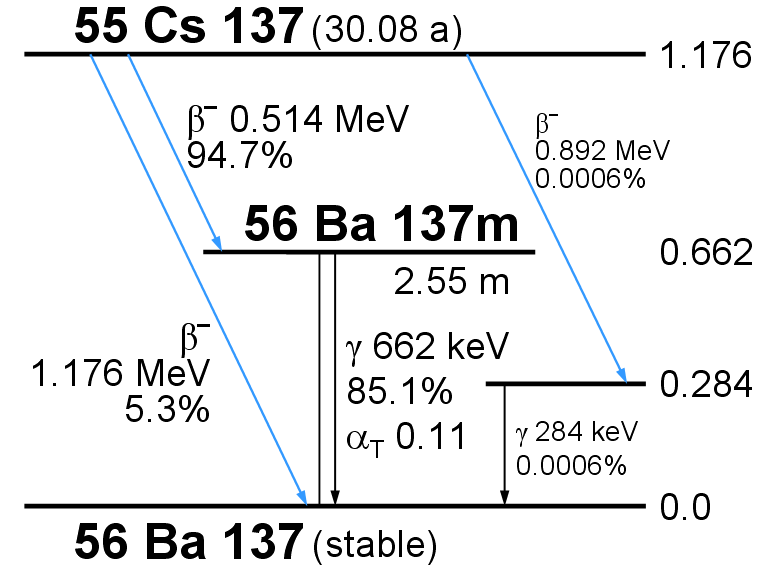
\includegraphics[width=\linewidth]{fig1(Cs_beta_decay)}
	\caption{Схема $\beta^{-}$-распада для $^{137}Cs$}
	\label{fig1:Cs_beta_decay}
\end{figure}

\pagebreak

\section*{Экспериментальная установка}

\begin{figure}[h]
	\centering
	\includegraphics[width=0.75\linewidth]{fig2(setup_1)}			
	\caption{Экспериментальная установка.(1) -- вакууметр ионизационно-термопарный, (2) -- источники питания катушки (магнитной линзы) }
	\label{fig2:setup_1}
\end{figure}

\begin{figure}[h]
	\centering
	\includegraphics[width=0.85\linewidth]{fig3(setup_2)}			
	\caption{Экспериментальная установка.(1) -- вентиль подключения форвакуумного насоса, (2) -- магнитная линза, (3) -- Счетчик}
	\label{fig3:setup_2}
\end{figure}

\begin{figure}[h]
	\centering
	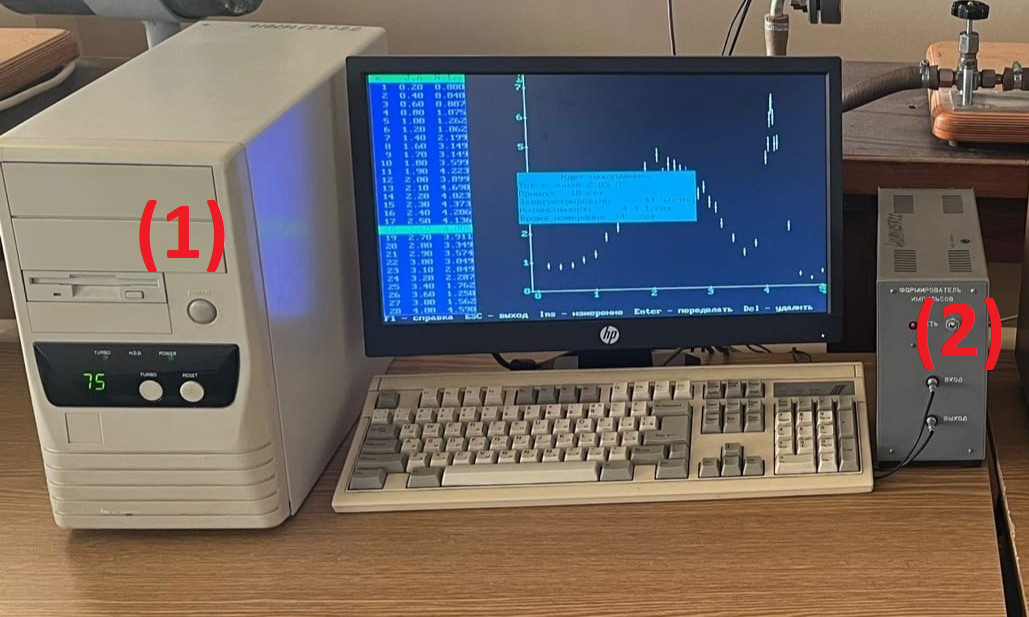
\includegraphics[width=0.8\linewidth]{fig4 (setup_3)}			
	\caption{Экспериментальная установка.(1) -- компьютер, показывающий спектр, (2) -- формирователь импульсов}
	\label{fig3:setup_2}
\end{figure}

\pagebreak

\section*{Ход работы}

Проведем измерение $\beta$-спектра, изменяя ток в магнитной линзе, будем измерять число попаданий частиц в детектор за 100 секунд. Также измерим фон и построим график зависимости количества попаданий частиц в детектор от тока, с учетом фона.

\begin{figure}[h!]
	\centering
	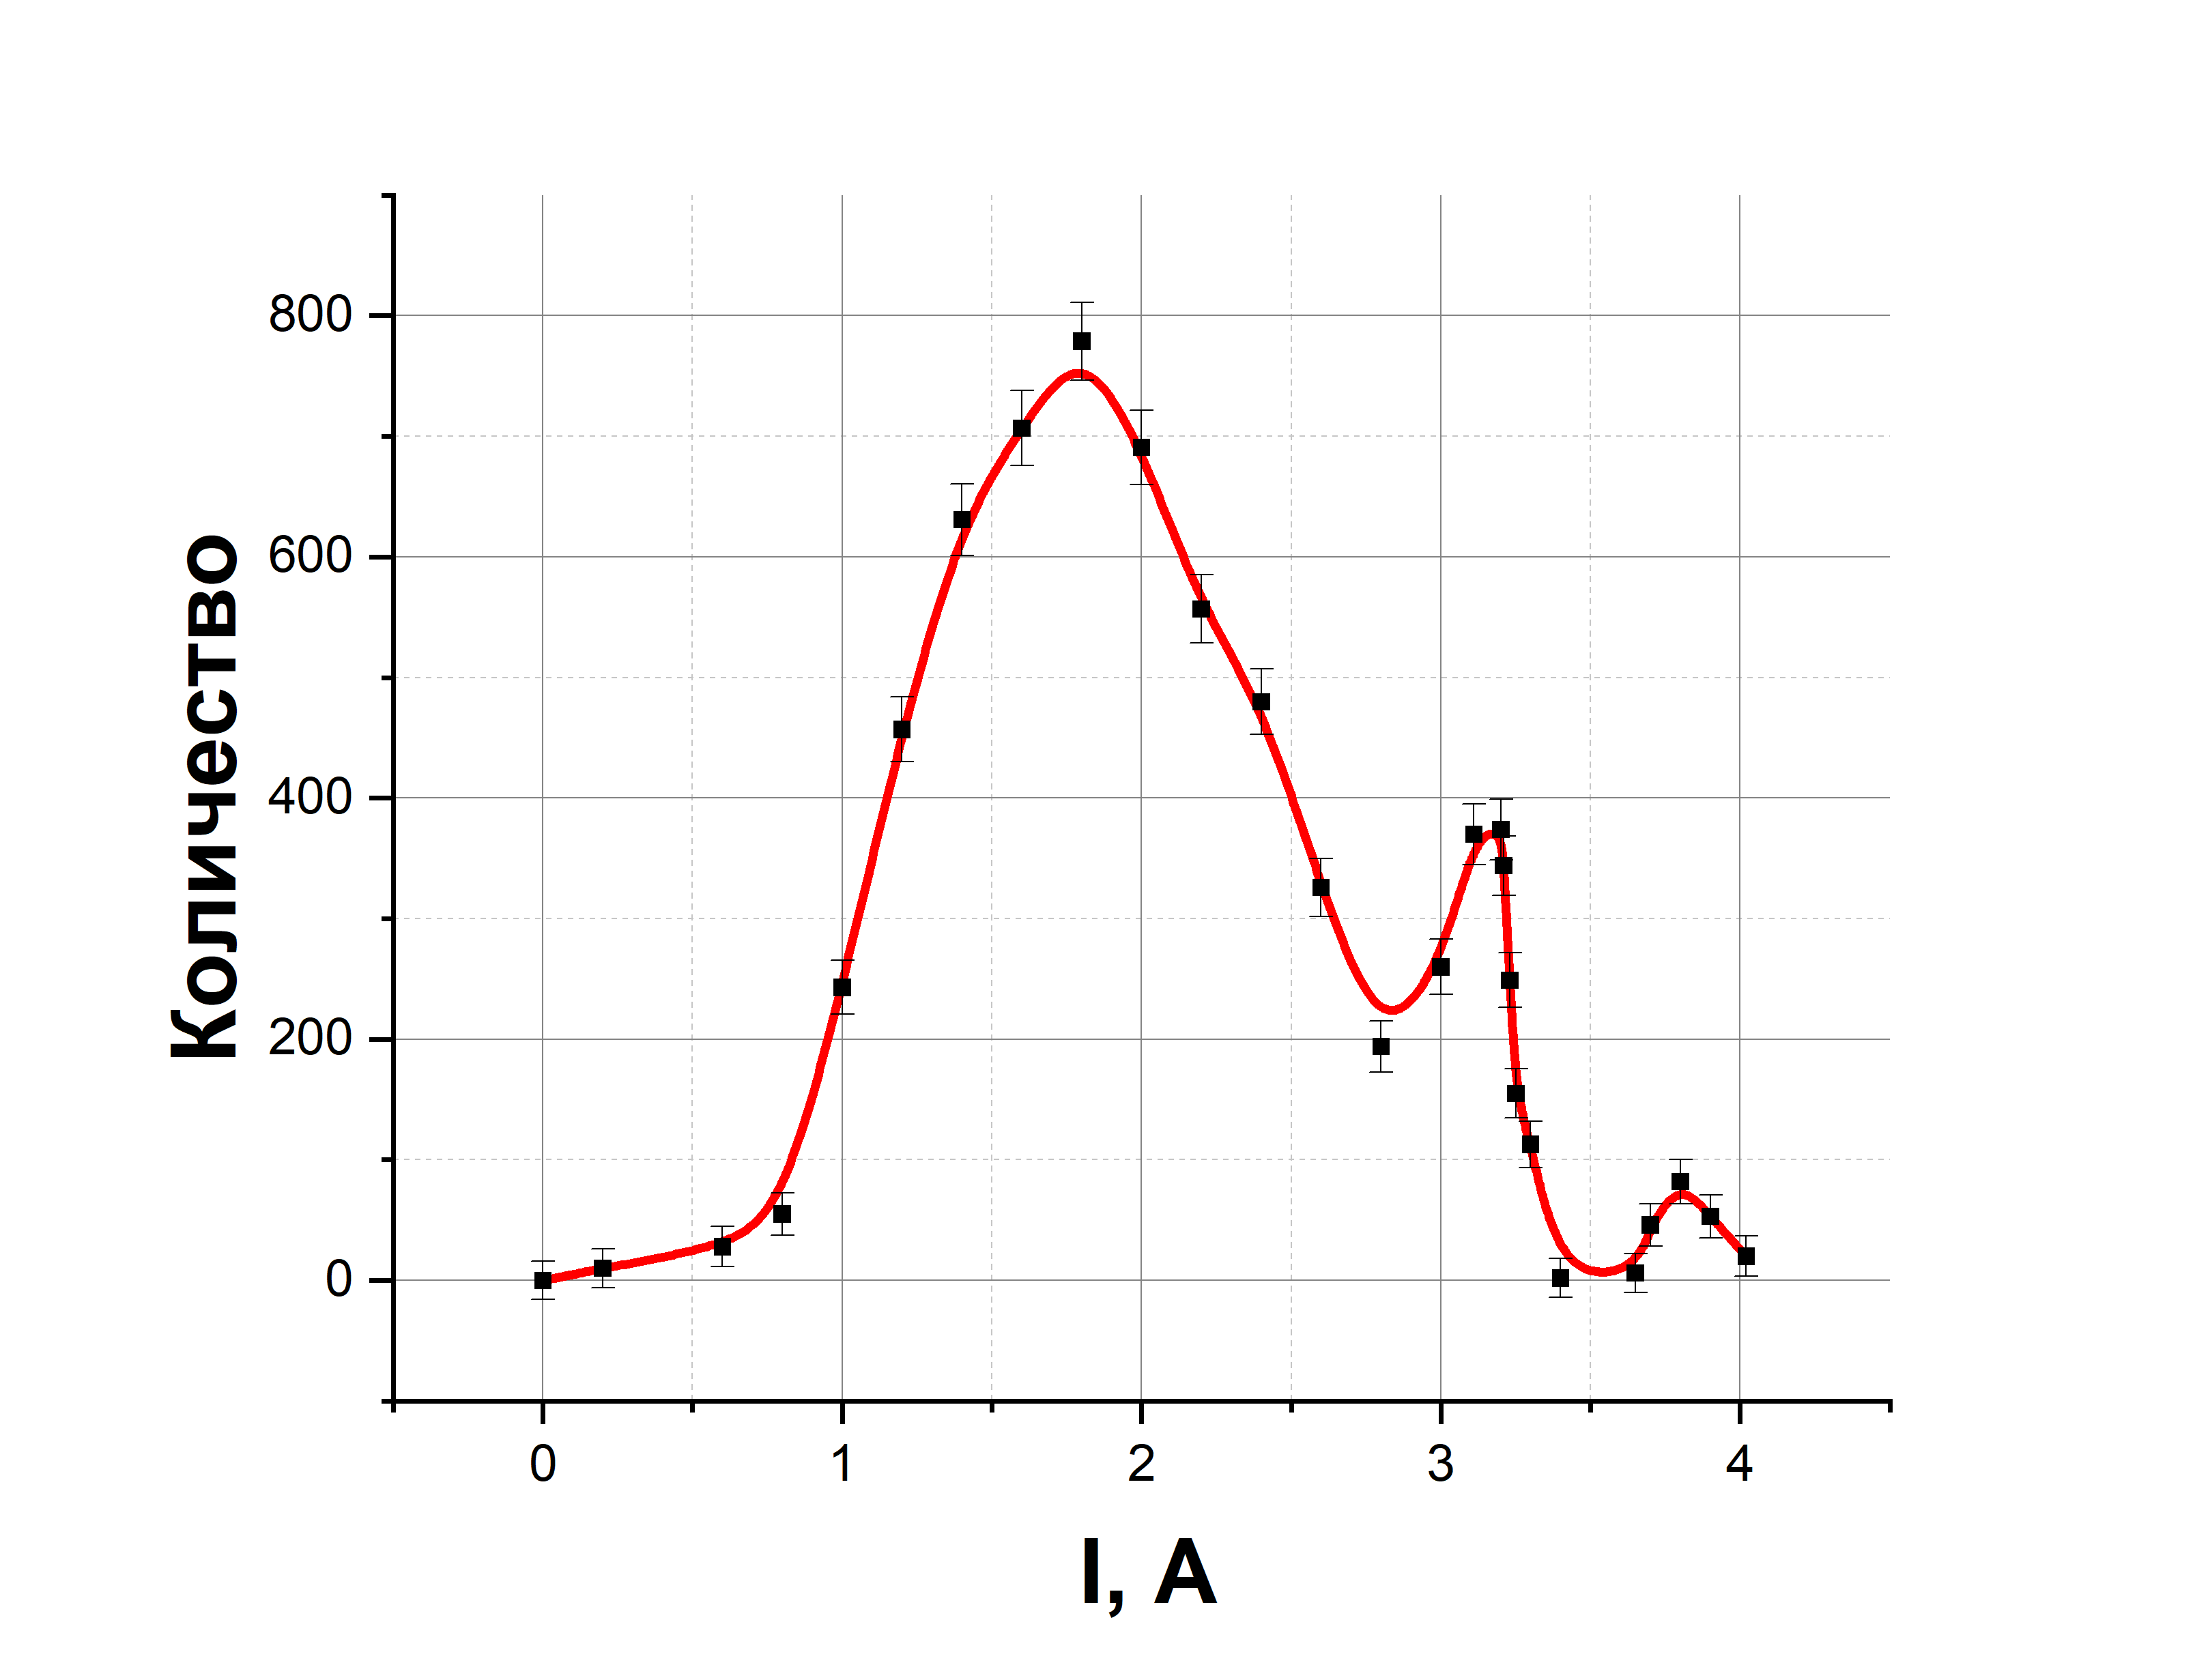
\includegraphics[width=0.9\linewidth]{graph1 (spectre)}
	\caption{Измеренный $\beta$-спектр $^{137}Cs$}
	\label{graph1:spectre}
\end{figure}

\pagebreak

Как известно из теории, $^{137} Cs$ должен иметь 1 узкий пик, соответствующий внутренней конверсии. Однако, как видно из Рисунка \ref{graph1:spectre}, мы получили 2 пика. 

Данное расхождение может быть связано с несовершенством экспериментальной установки, а именно, в <<сбитом фокусе>> магнитной линзы.

Проанализируем каждый пик отдельно. Согласно статистическим законам, оба пика должны иметь форму Гауссовой кривой, найдем параметры данной кривой.

\begin{figure}[h!]
	\centering
	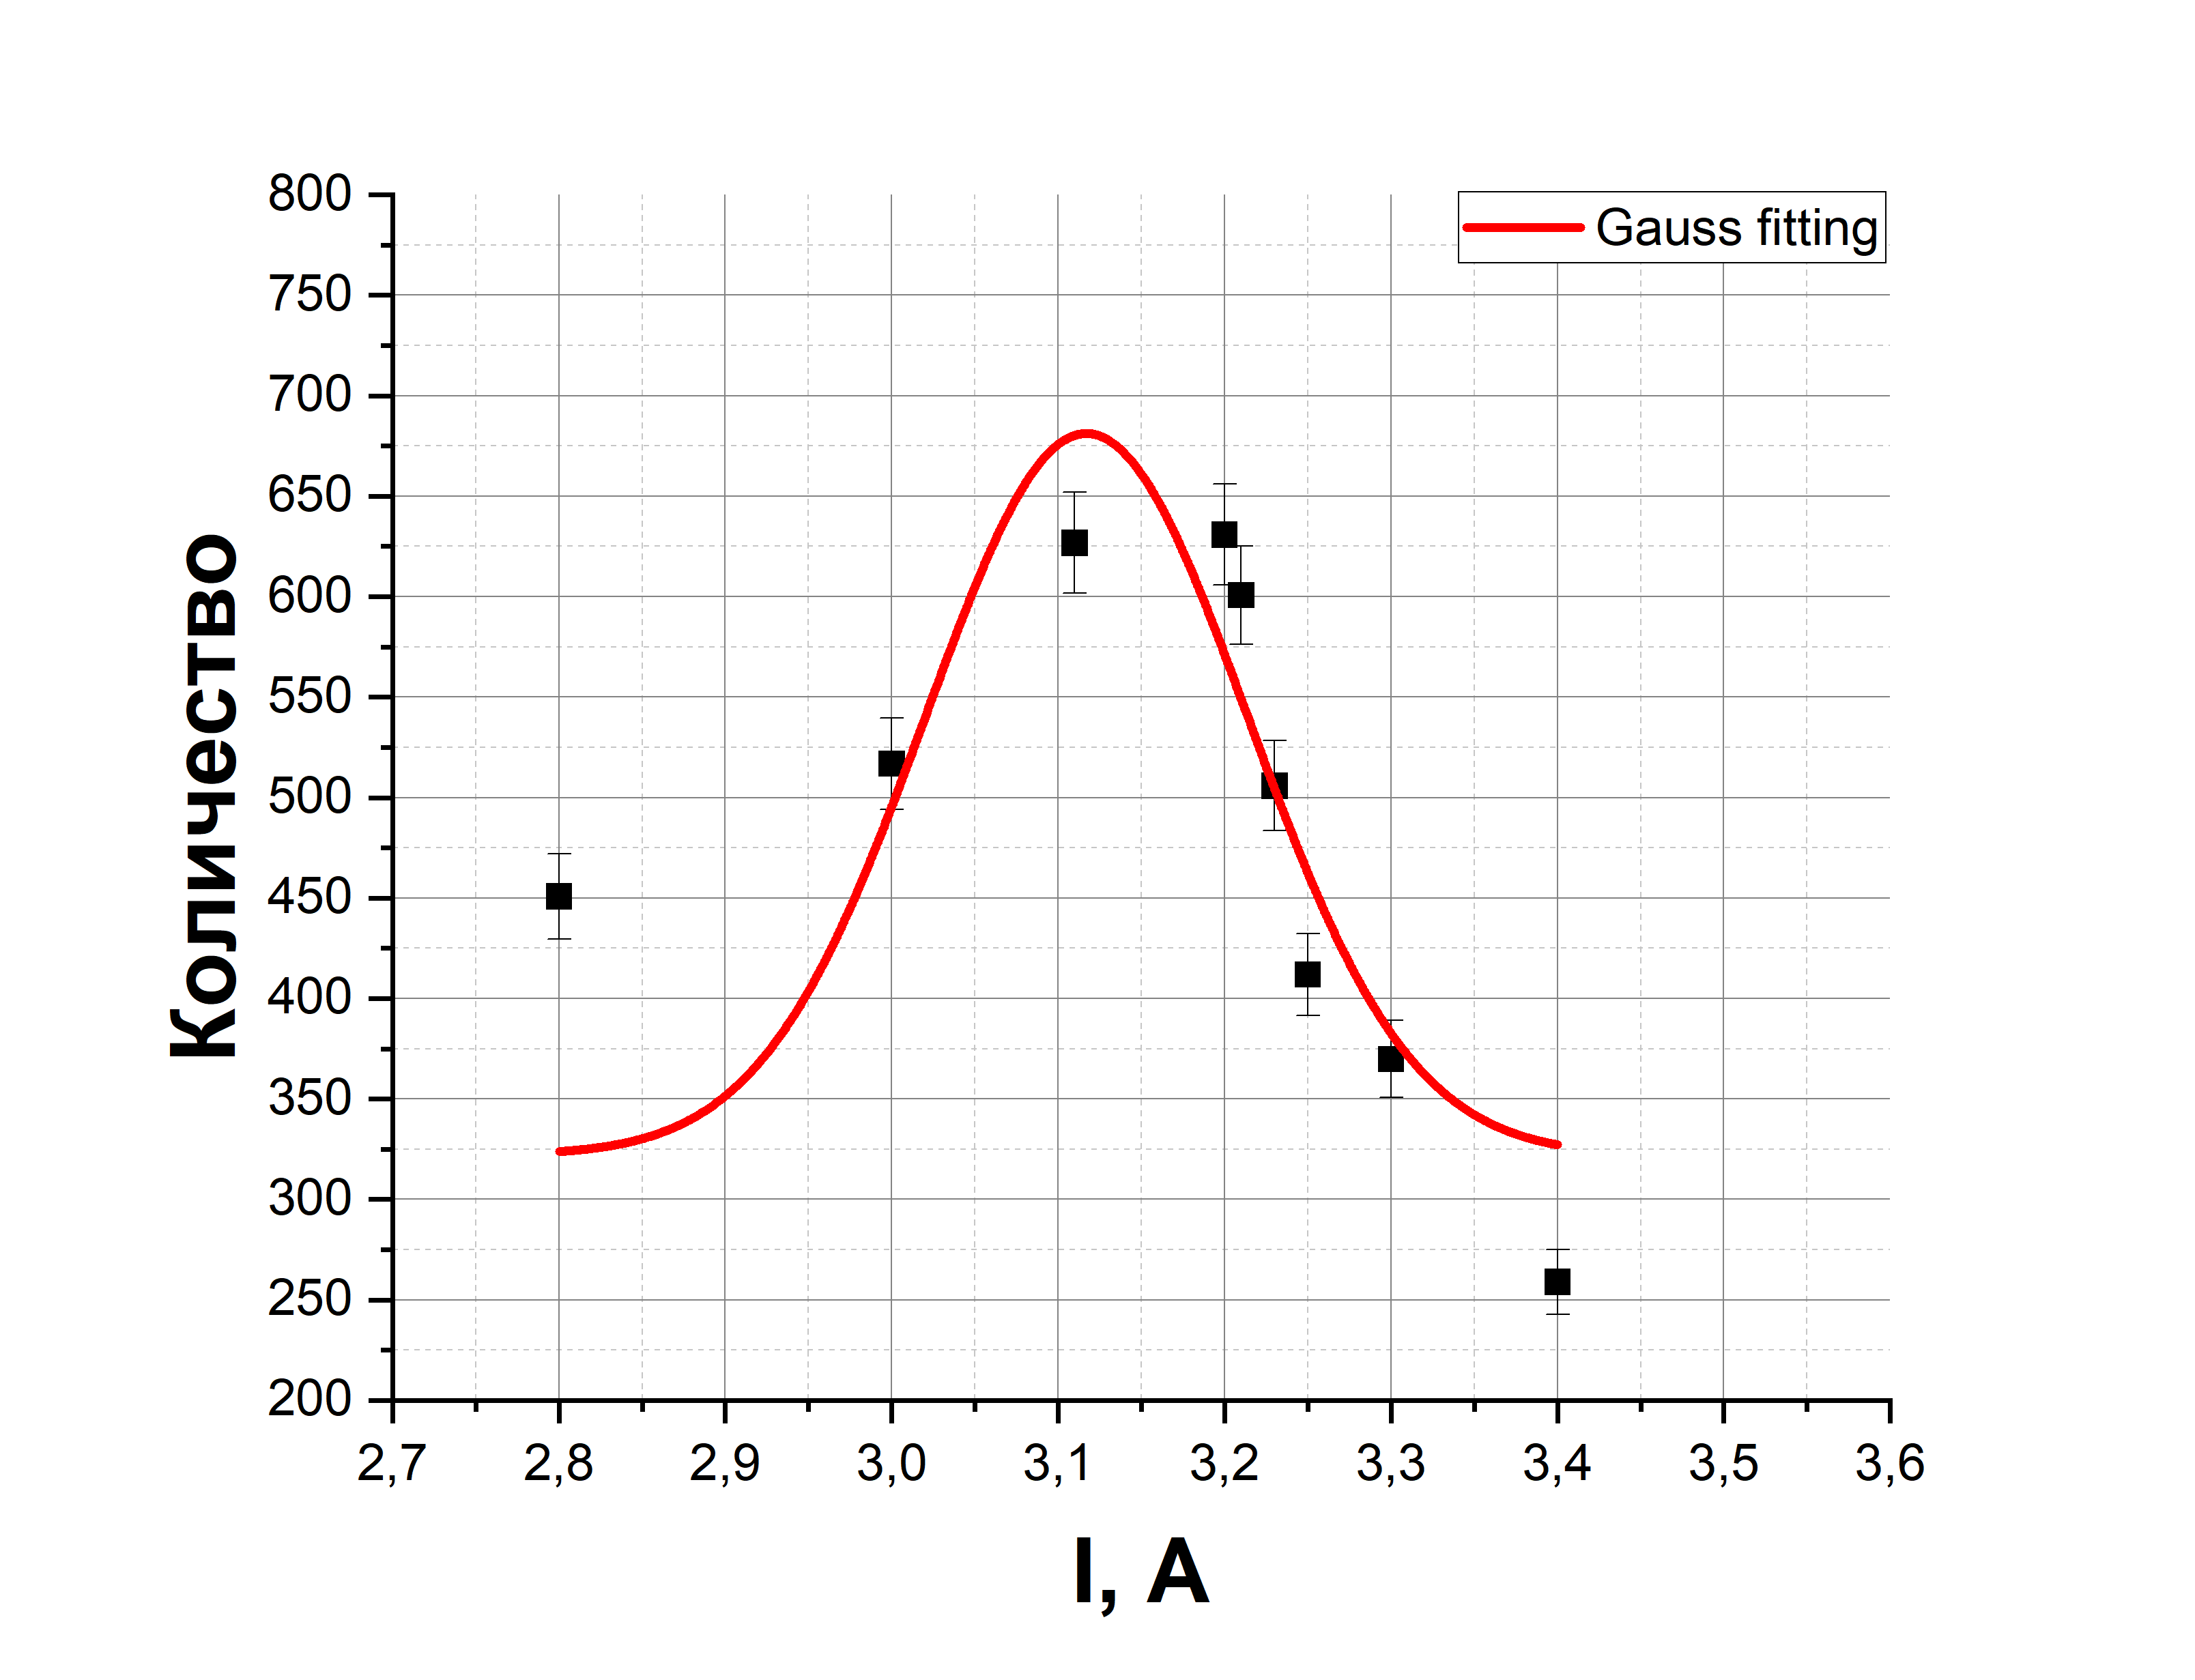
\includegraphics[width=0.75\linewidth]{graph2 (Gauss_1)}
	\caption{Первый Гауссов пик $\beta$-спектре $^{137}Cs$}
	\label{graph2:Gauss_1}
\end{figure}

\begin{figure}[h!]
	\centering
	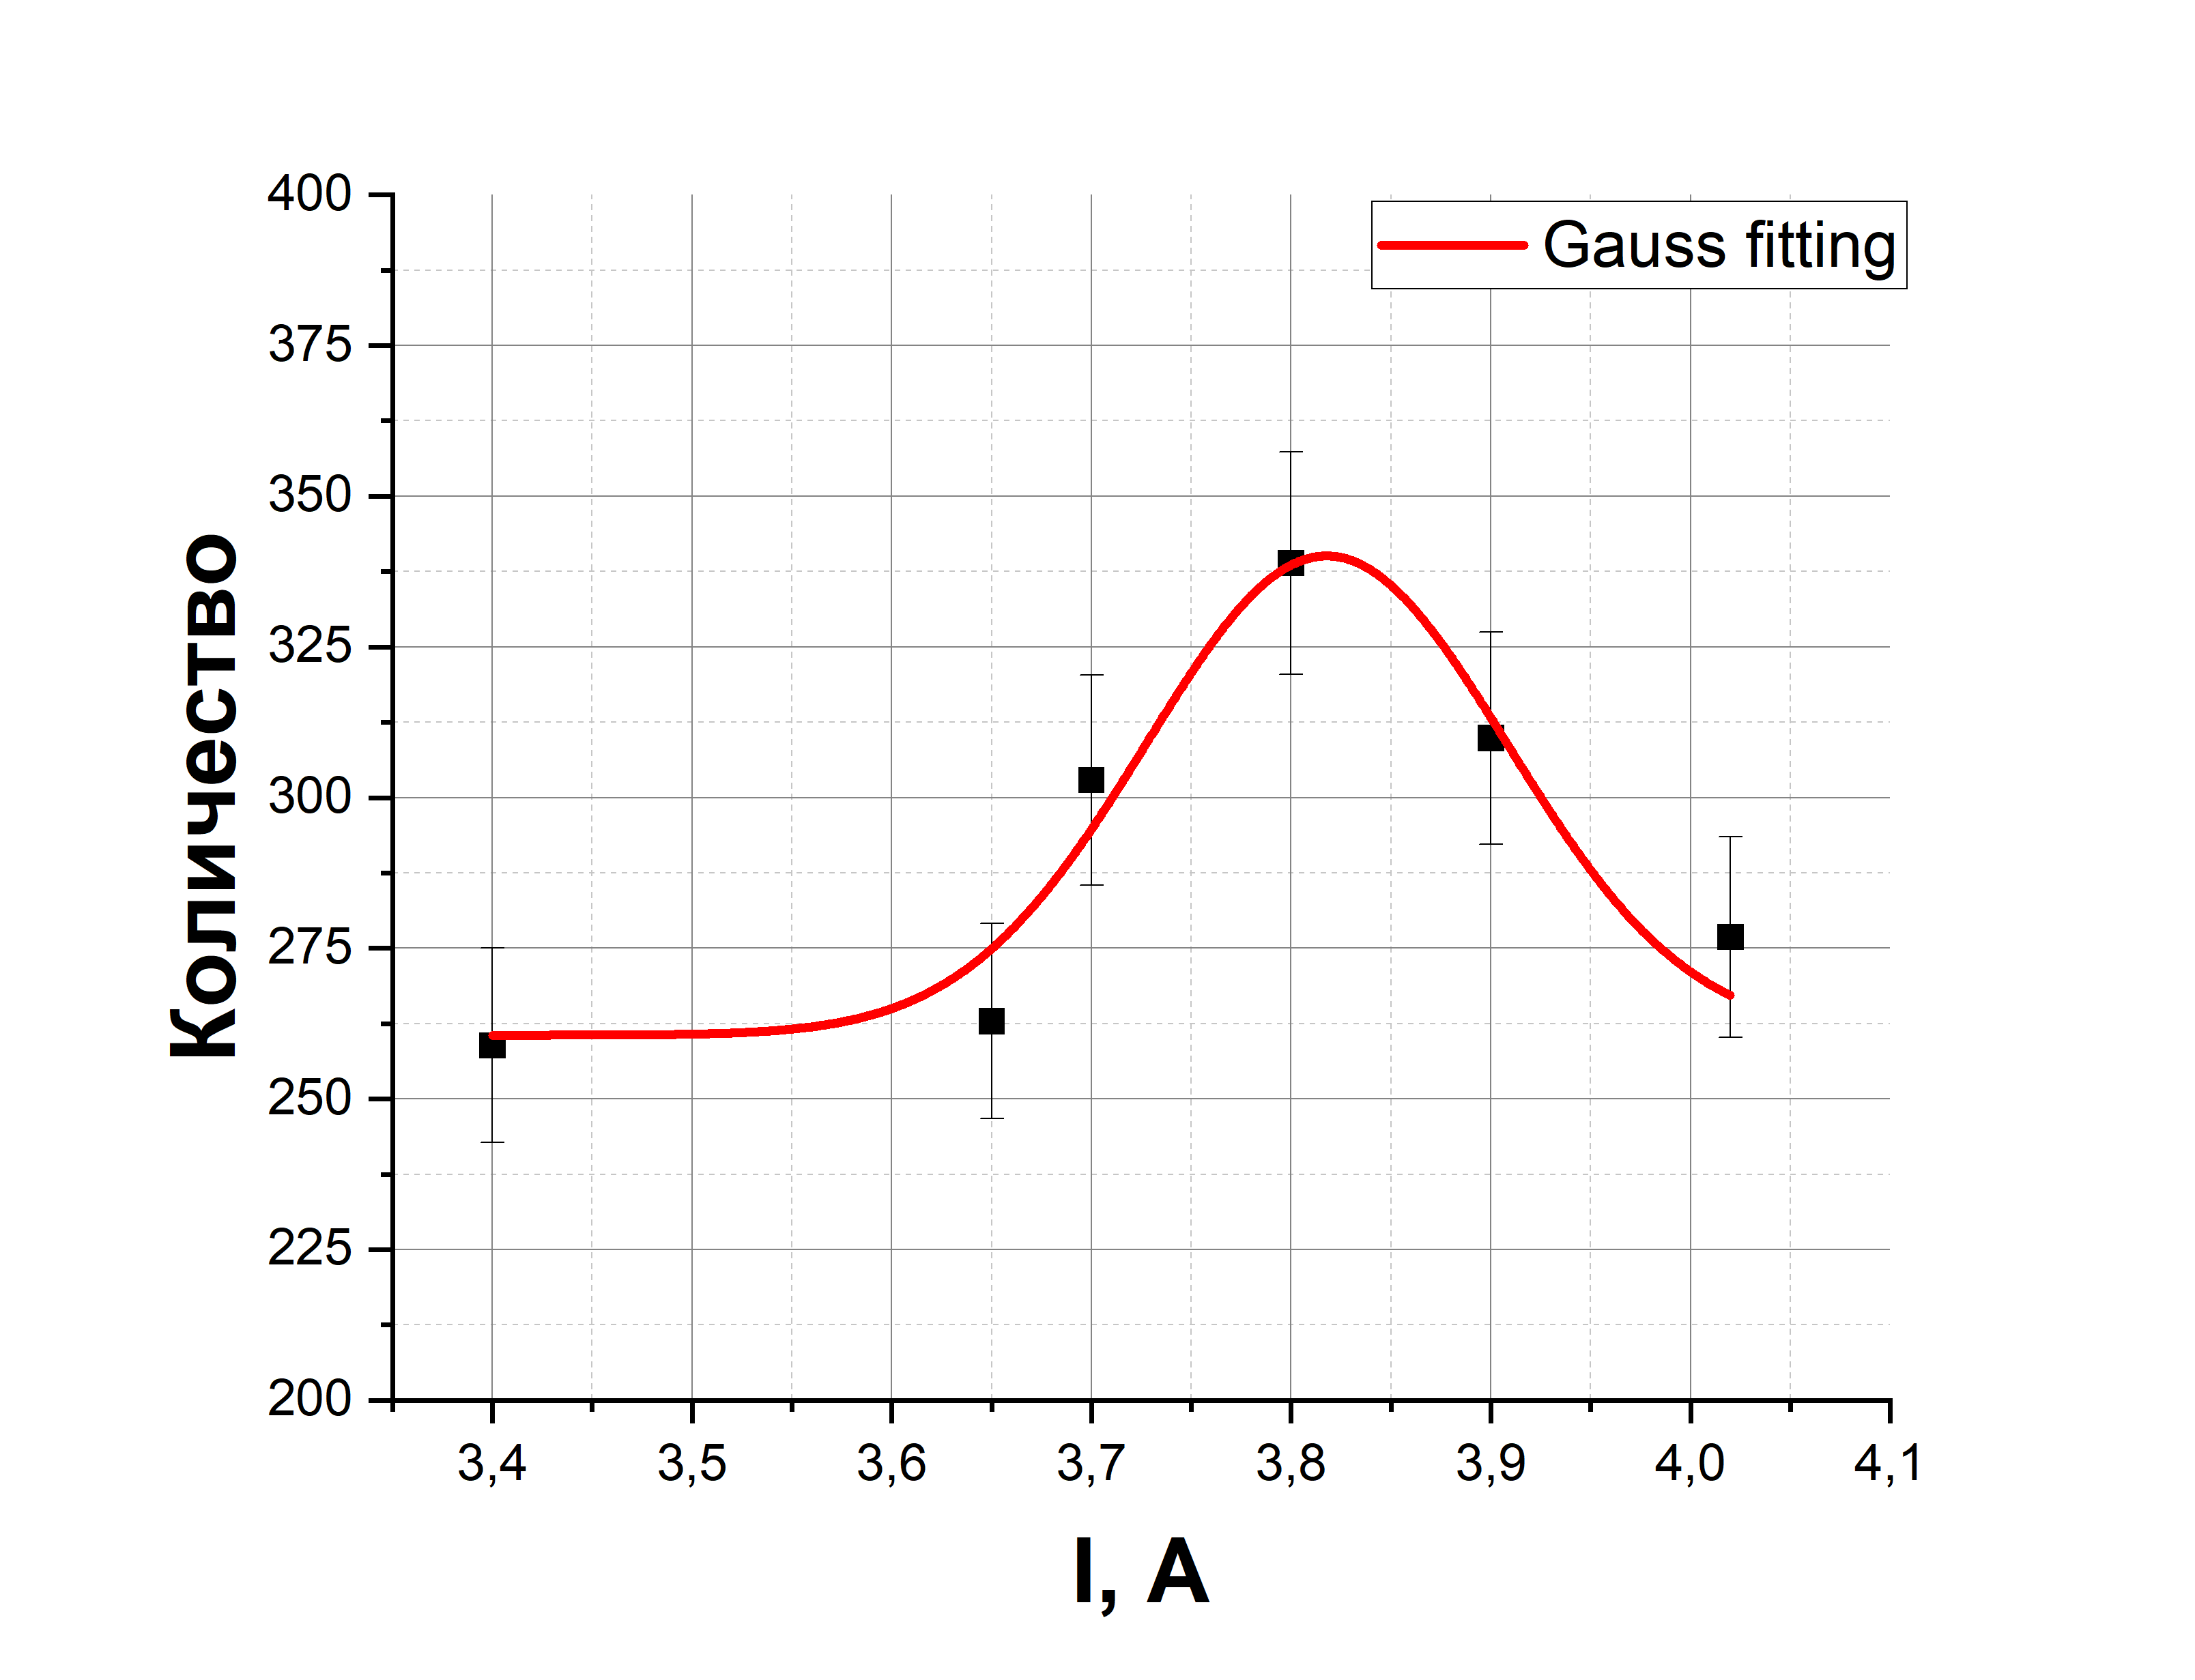
\includegraphics[width=0.75\linewidth]{graph3 (Gauss_2)}
	\caption{Второй Гауссов пик в $\beta$-спектре $^{137}Cs$}
	\label{graph1:Gauss_2}
\end{figure}

\pagebreak

Предполагая, что каждый из данных пиков соответствует внутренней конверсии $^{137}Cs$ (раздвоенное изображение из-за несовершенства магнитной линзы), зная положение каждого из пиков и энергию электронов внутренней конверсии $^{137}Cs$, мы сможем найти коэффициент пропорциональности тока и импульса электрона.

\begin{align*}
	k_1 = (326,9 \pm 12,1) \ кЭв / (A*с) \\
	k_2 = (266,7 \pm 7,1) \ кЭв / (A*с) \\
\end{align*}

, где $c$ -- скорость света.

Будем считать, что график на Рисунке \ref{graph1:spectre} является линейной комбинацией двух функций. Аппроксимируем первый общий пик такой линейной комбинацией, она имеет вид:

\begin{align} \label{eq2:exp_func}
	N(I) = c \times (k_1 I)^3 \left( \sqrt{a^2 + 511^2}-\sqrt{(k_1 I)^2 + 511^2} \right)^2 + d \times (k_2 I)^3 \left(\sqrt{a^2+511^2} -\sqrt{(k_2 I)^2 + 511^2}\right)^2 
\end{align}

, где a,c,d -- варьируемые параметры($a = p^2_{max}c^2$).

Полученный график изображен на Рисунок \ref{graph4:spectre_approx}


\begin{figure}[h!]
	\centering
	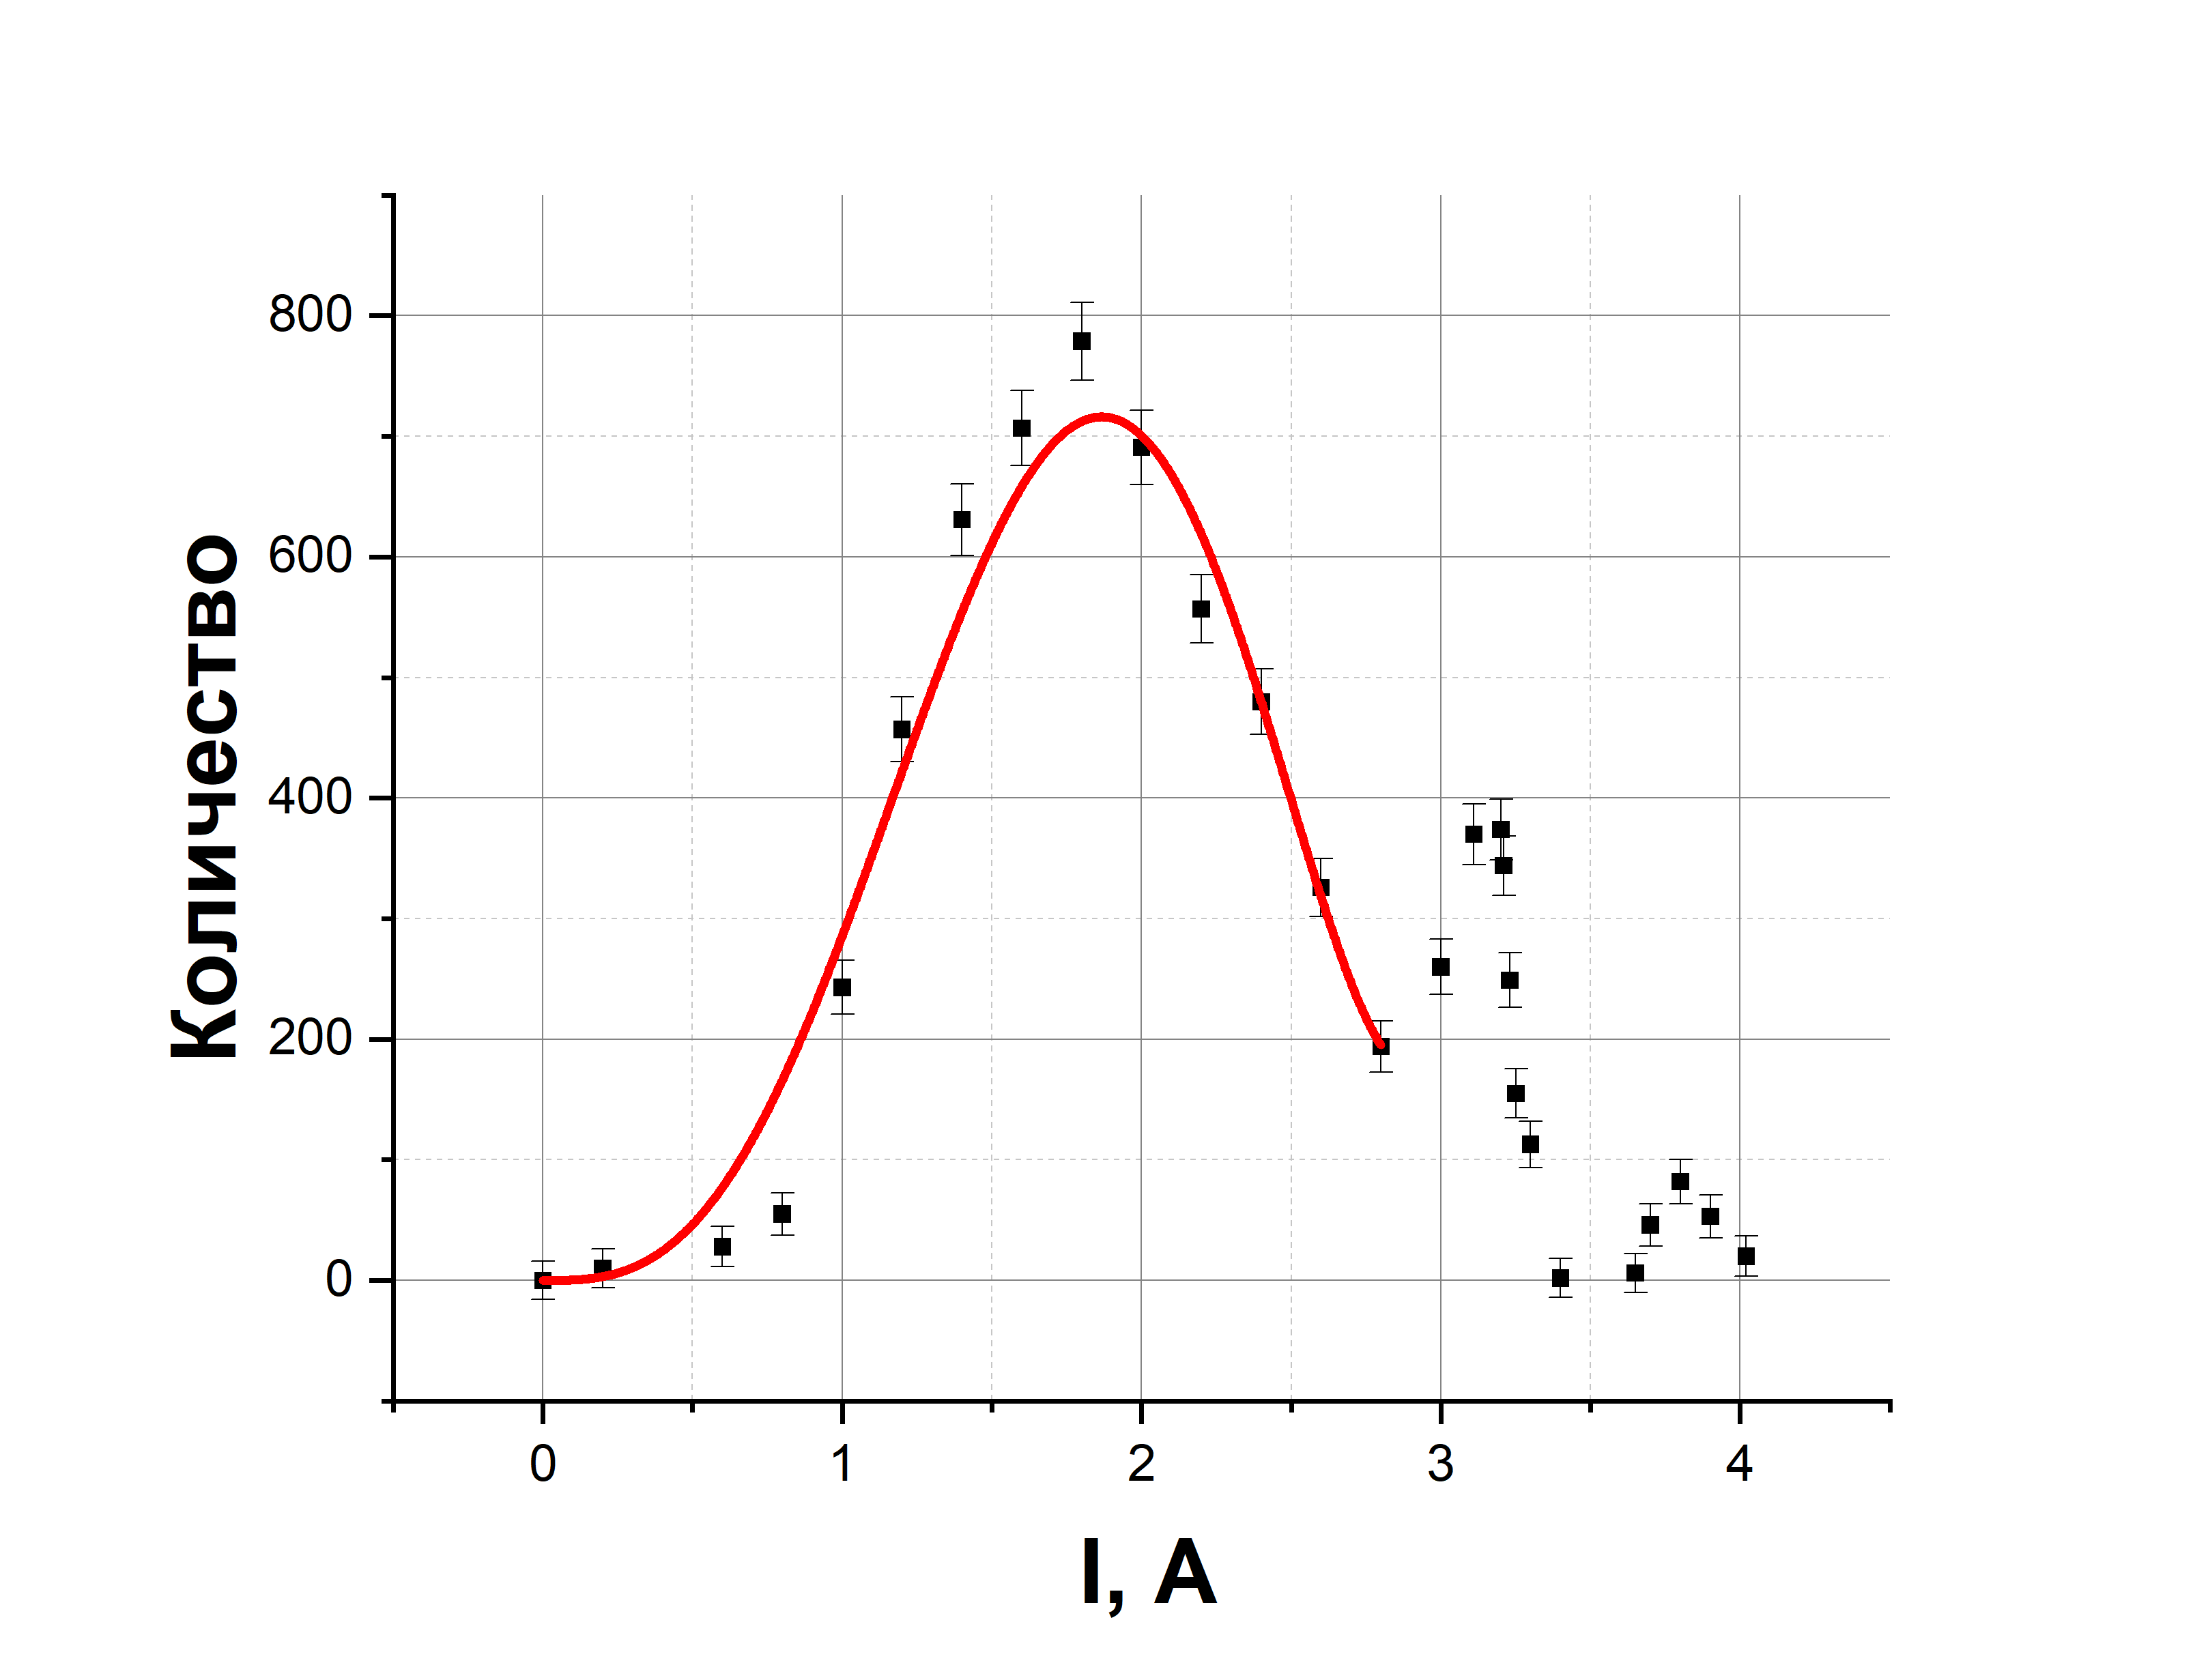
\includegraphics[width=\linewidth]{graph4 (spectre_approx_3)}
	\caption{Аппроксимация $\beta$-спектра $^{137}Cs$}
	\label{graph4:spectre_approx}
\end{figure}

\pagebreak

Из аппроксимации получим параметр а, тем самым мы сможем рассчитать максимальную энергию.

\begin{align*}
	T_{max} = \sqrt{p^2_{max} c^2 + m^2 c^4} - mc^2  \approx (535 \pm 40) \ кЭв
\end{align*}


Зависимость \ref{eq2:exp_func} можно записать в терминах энергии:

\begin{align*}
	N(I)/I^3 = c*k_1^3 (T_{max} - T_1)^2 + d*k_2^3 (T_{max} - T_2)^2 = f(T_1, T_2)
\end{align*}

Зная параметры c, d из предыдущей аппроксимации построим зависимость $f(T_1, T_2)$,$T_{max}$ возьмем как параметр аппроксимации.

\begin{figure}[h!]
	\centering
	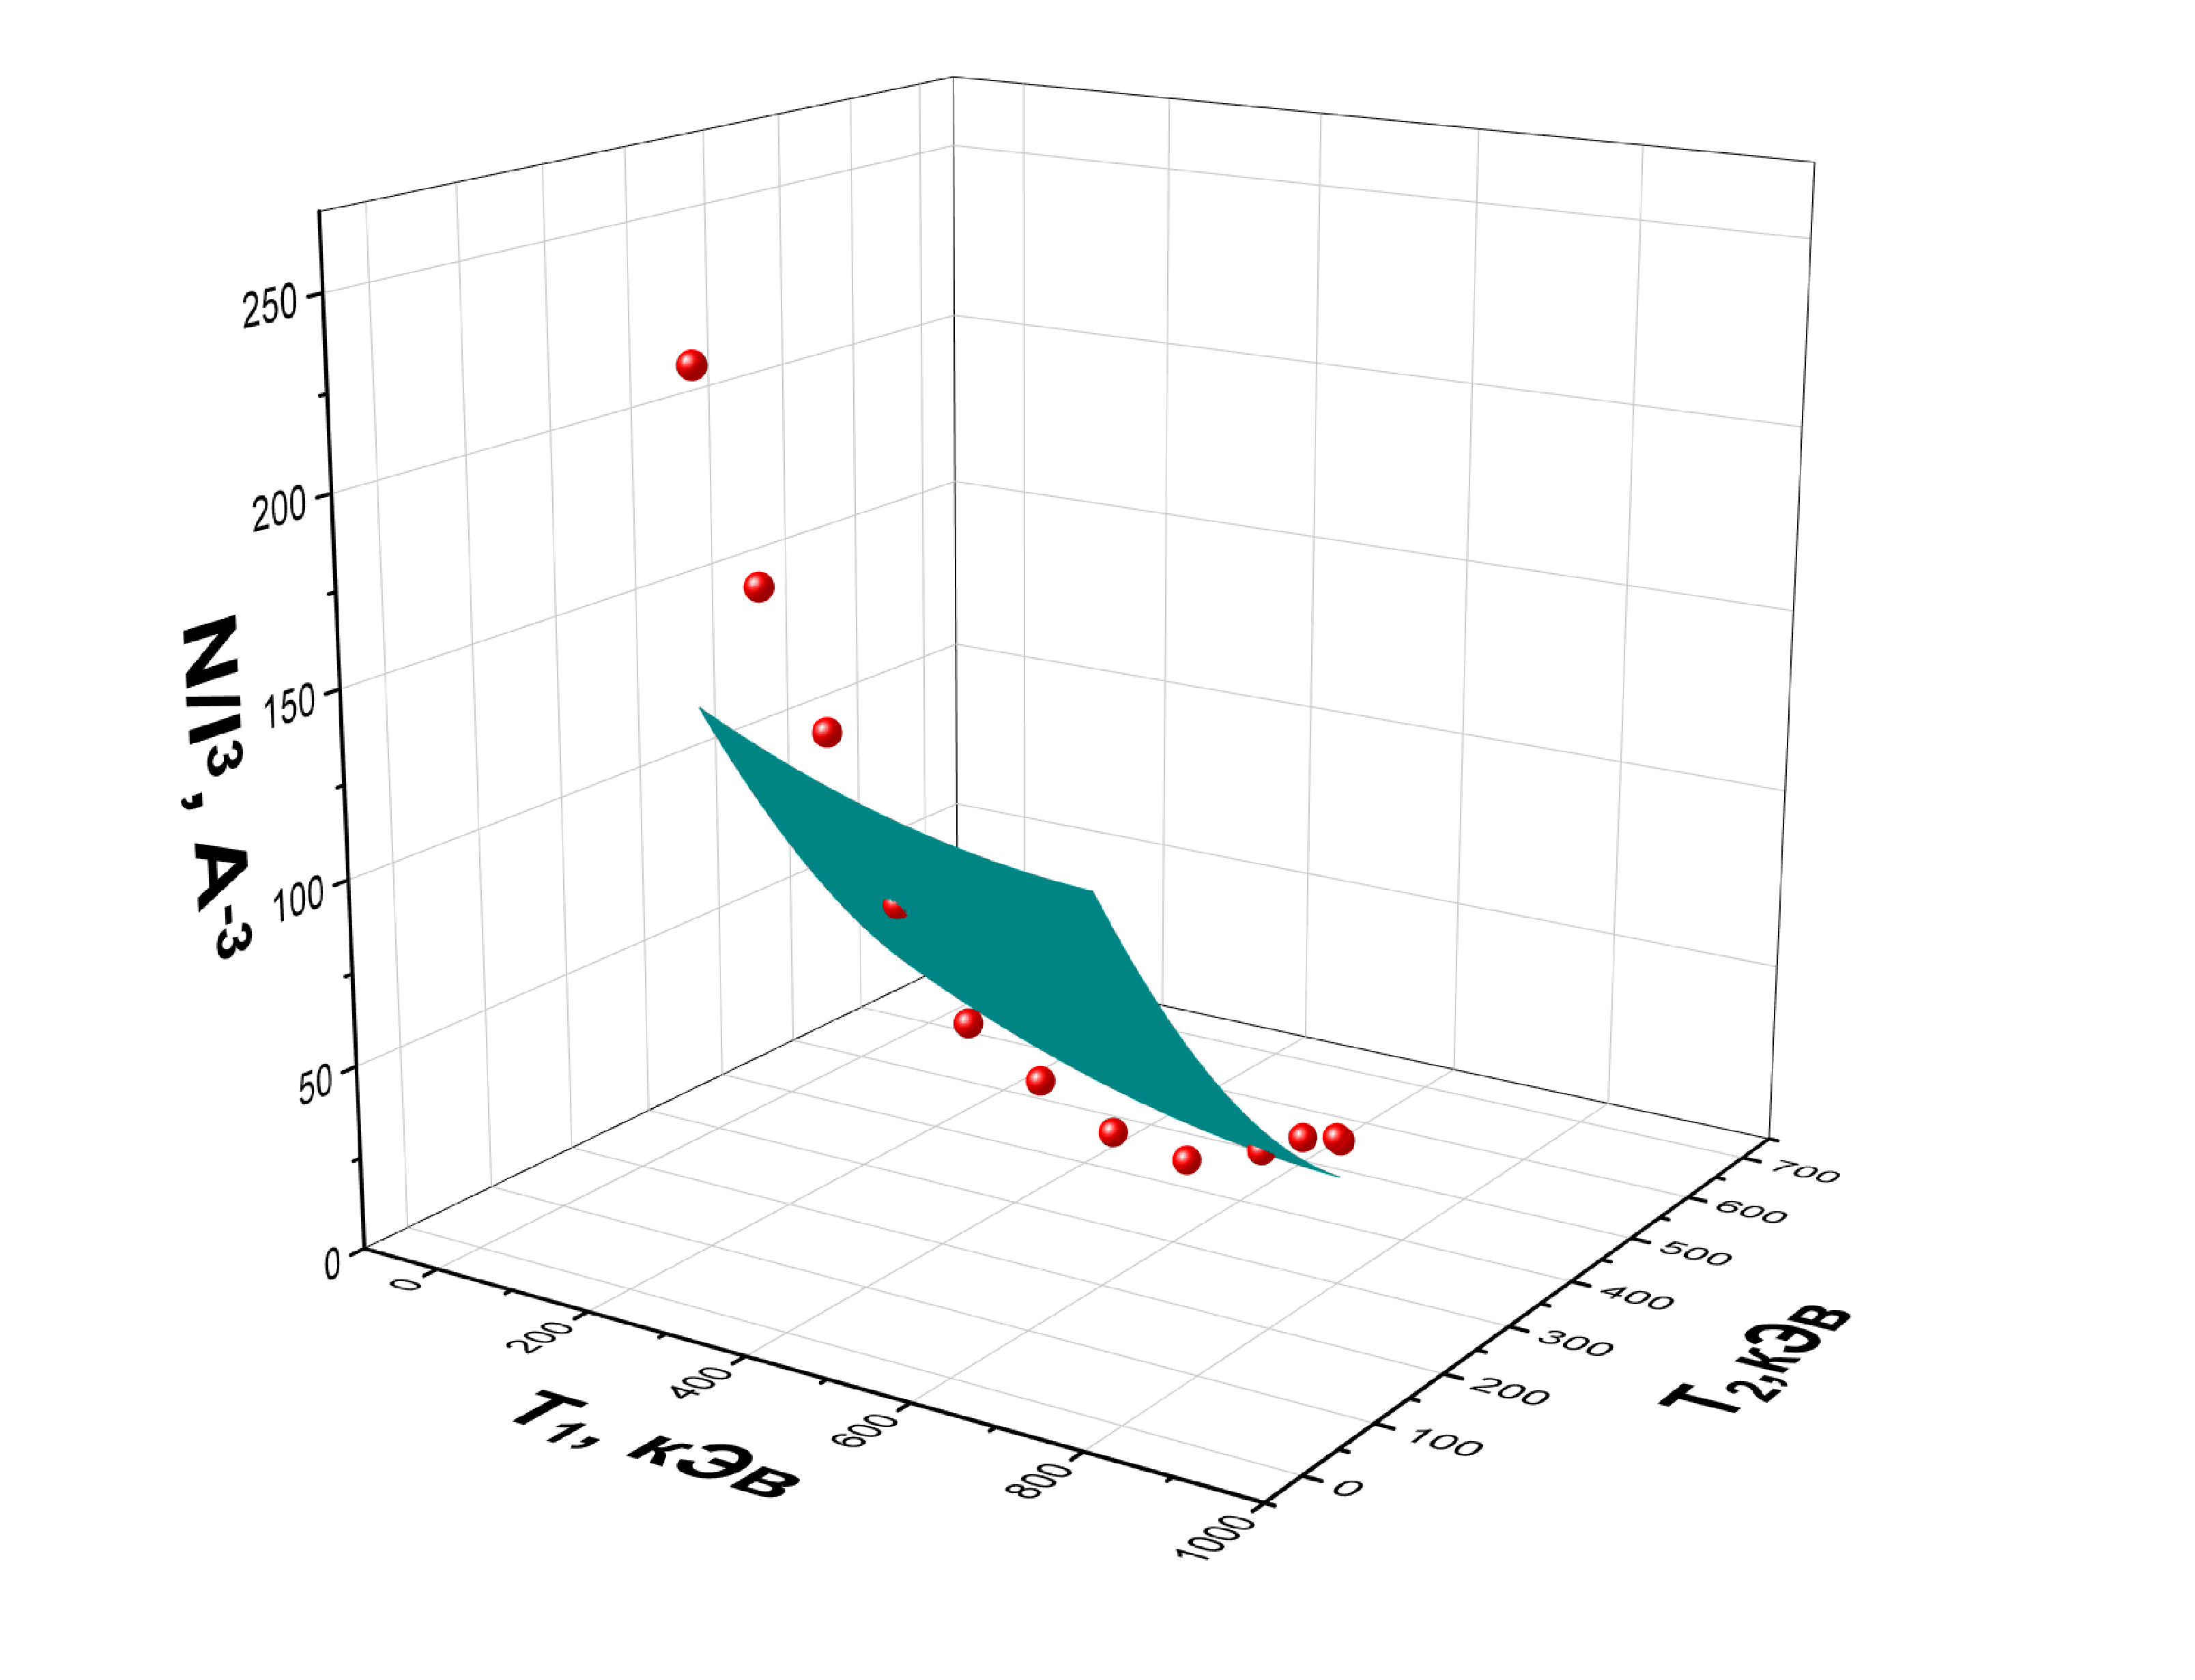
\includegraphics[width=\linewidth]{graph5 (3D_approx)}
	\caption{Аппроксимация функции $\frac{N}{I^3}(T_1, T_2)$}
	\label{graph4:spectre_approx}
\end{figure}

Результат аппроксимации -- $T_{max} = 698 \ кЭв$. Визуально оценим погрешности. Построим еще поверхности, аппроксимирующие данных точки, чтобы понять пределы погрешности для $T_{max}$

\newpage

\begin{figure}[h!]
	\centering
	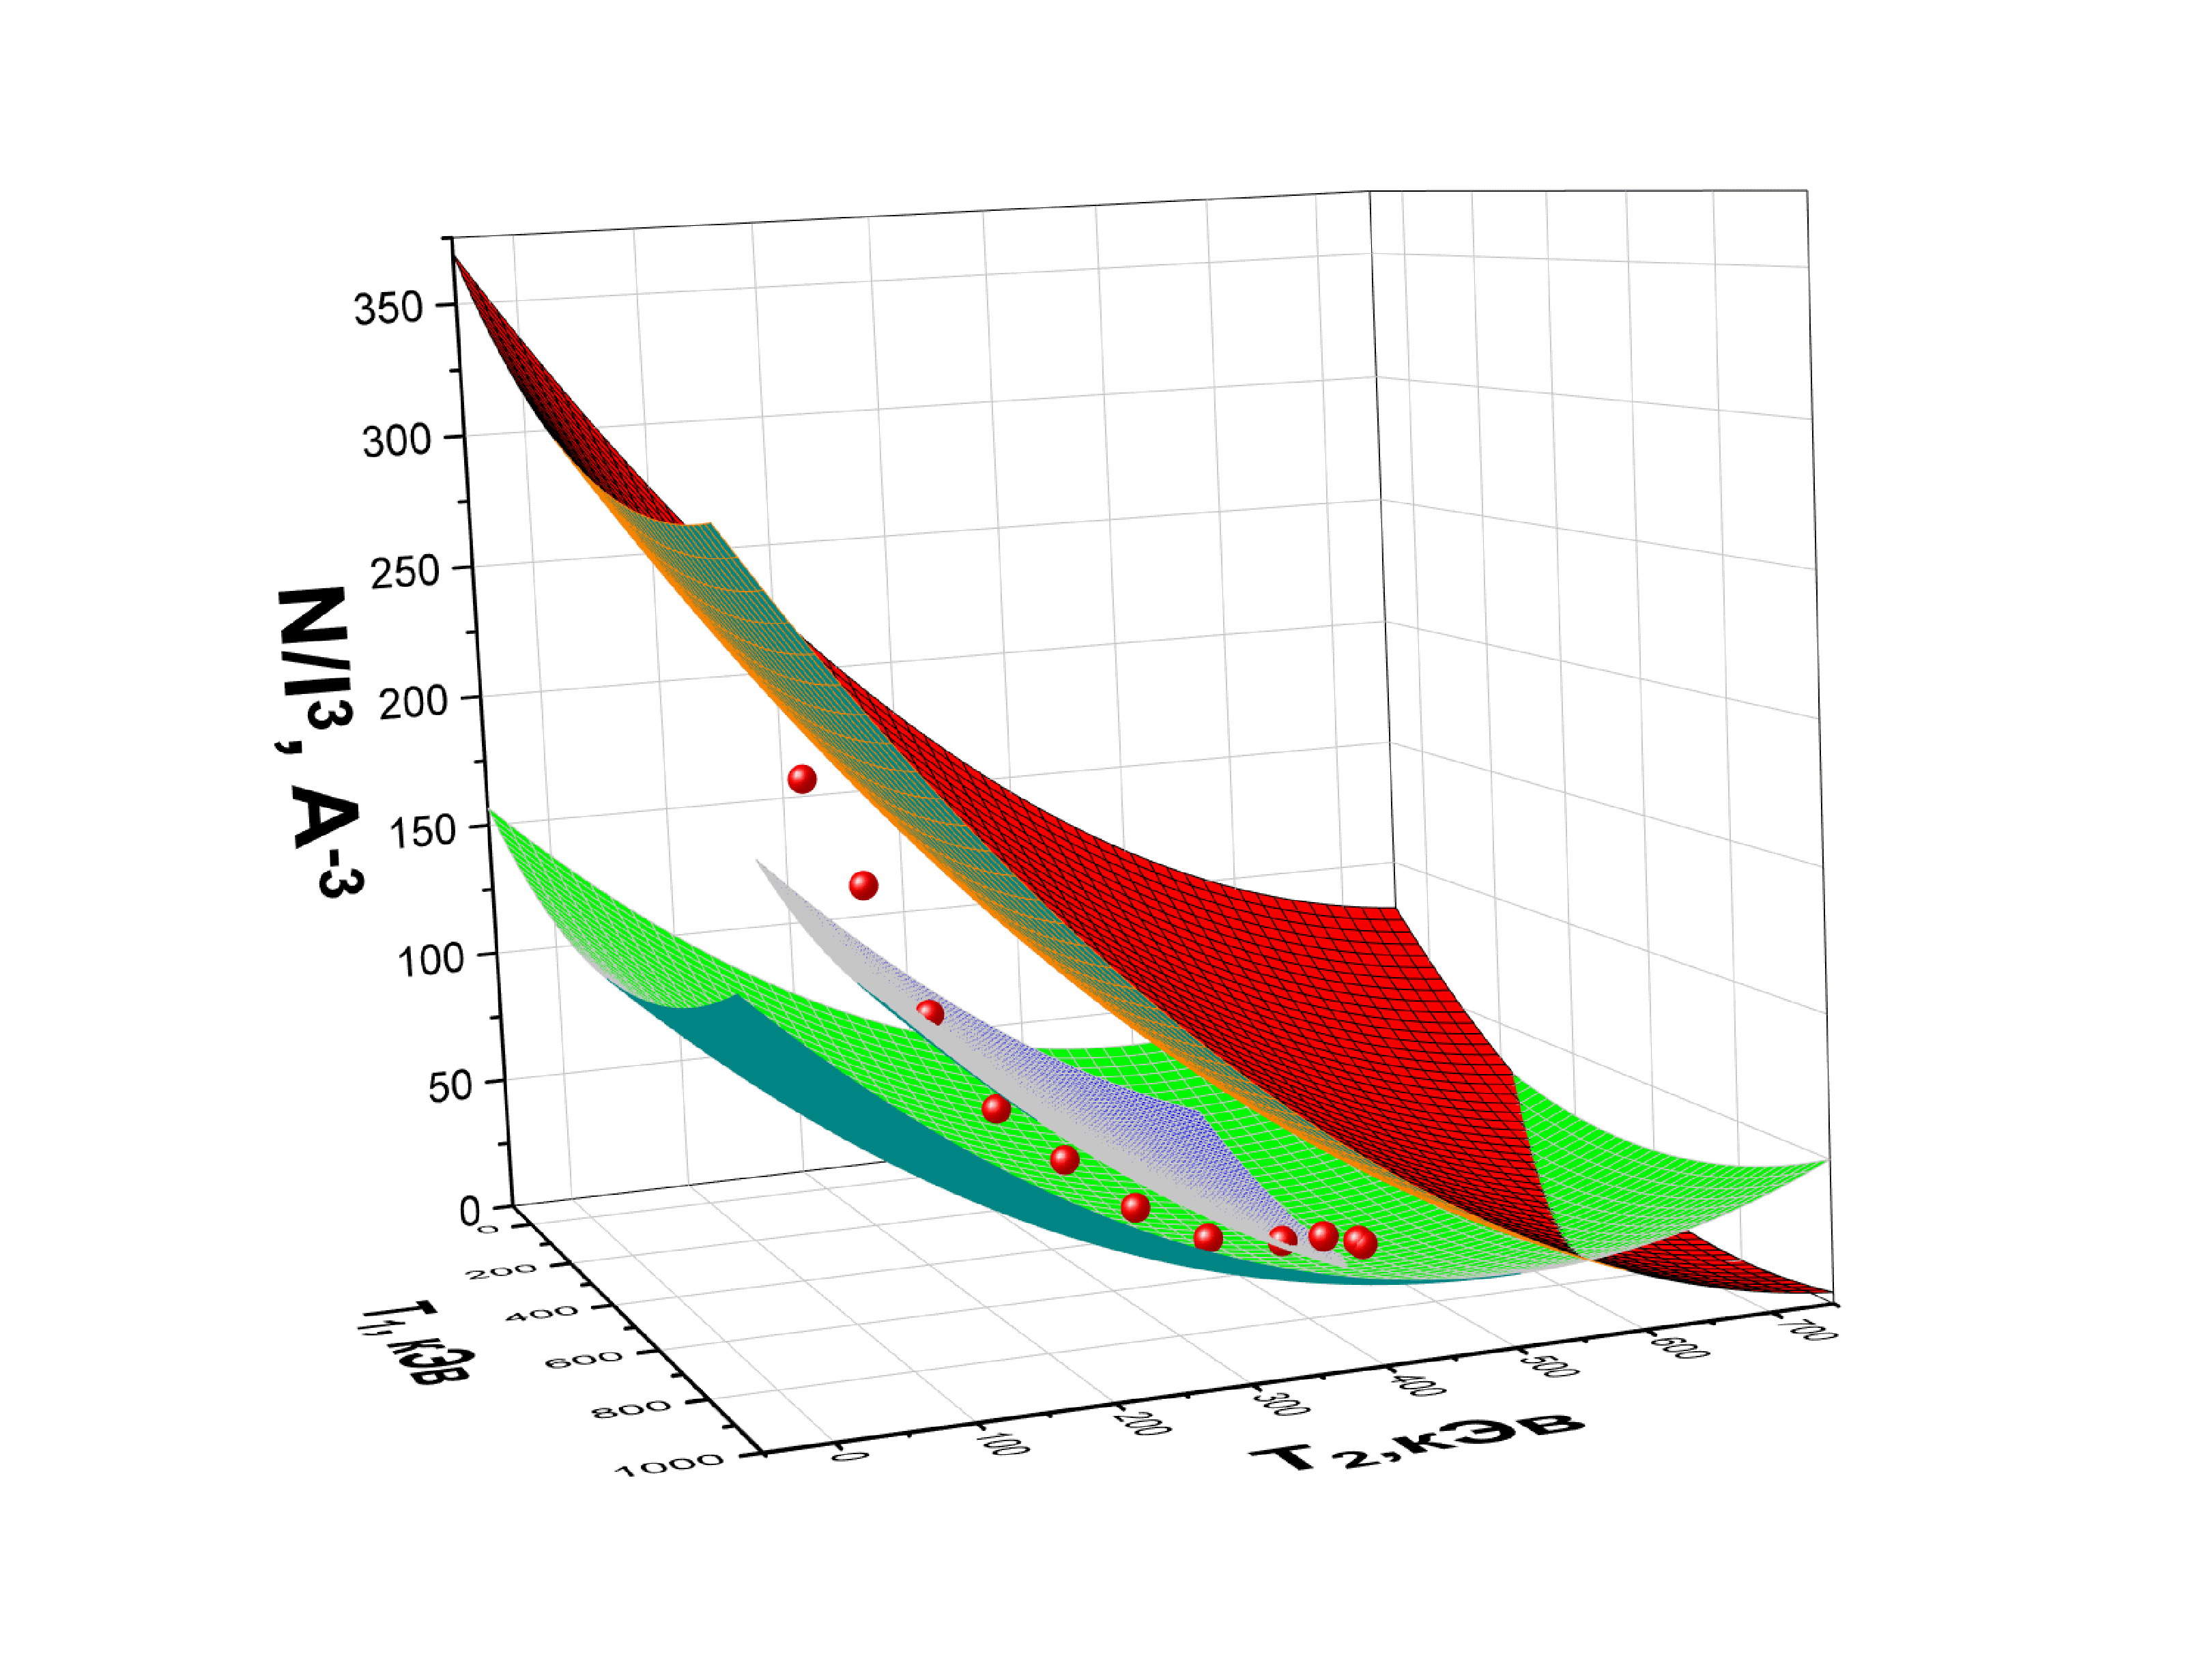
\includegraphics[width=0.8\linewidth]{graph6}
	\caption{Графики, для оценки погрешности $T_{max}$. Верхняя кривая -- $T_{max} = 800 \ кЭв$, нижняя -- $T_{max} = 500 \ кЭв$}
\end{figure}

\begin{figure}[h!]
	\centering
	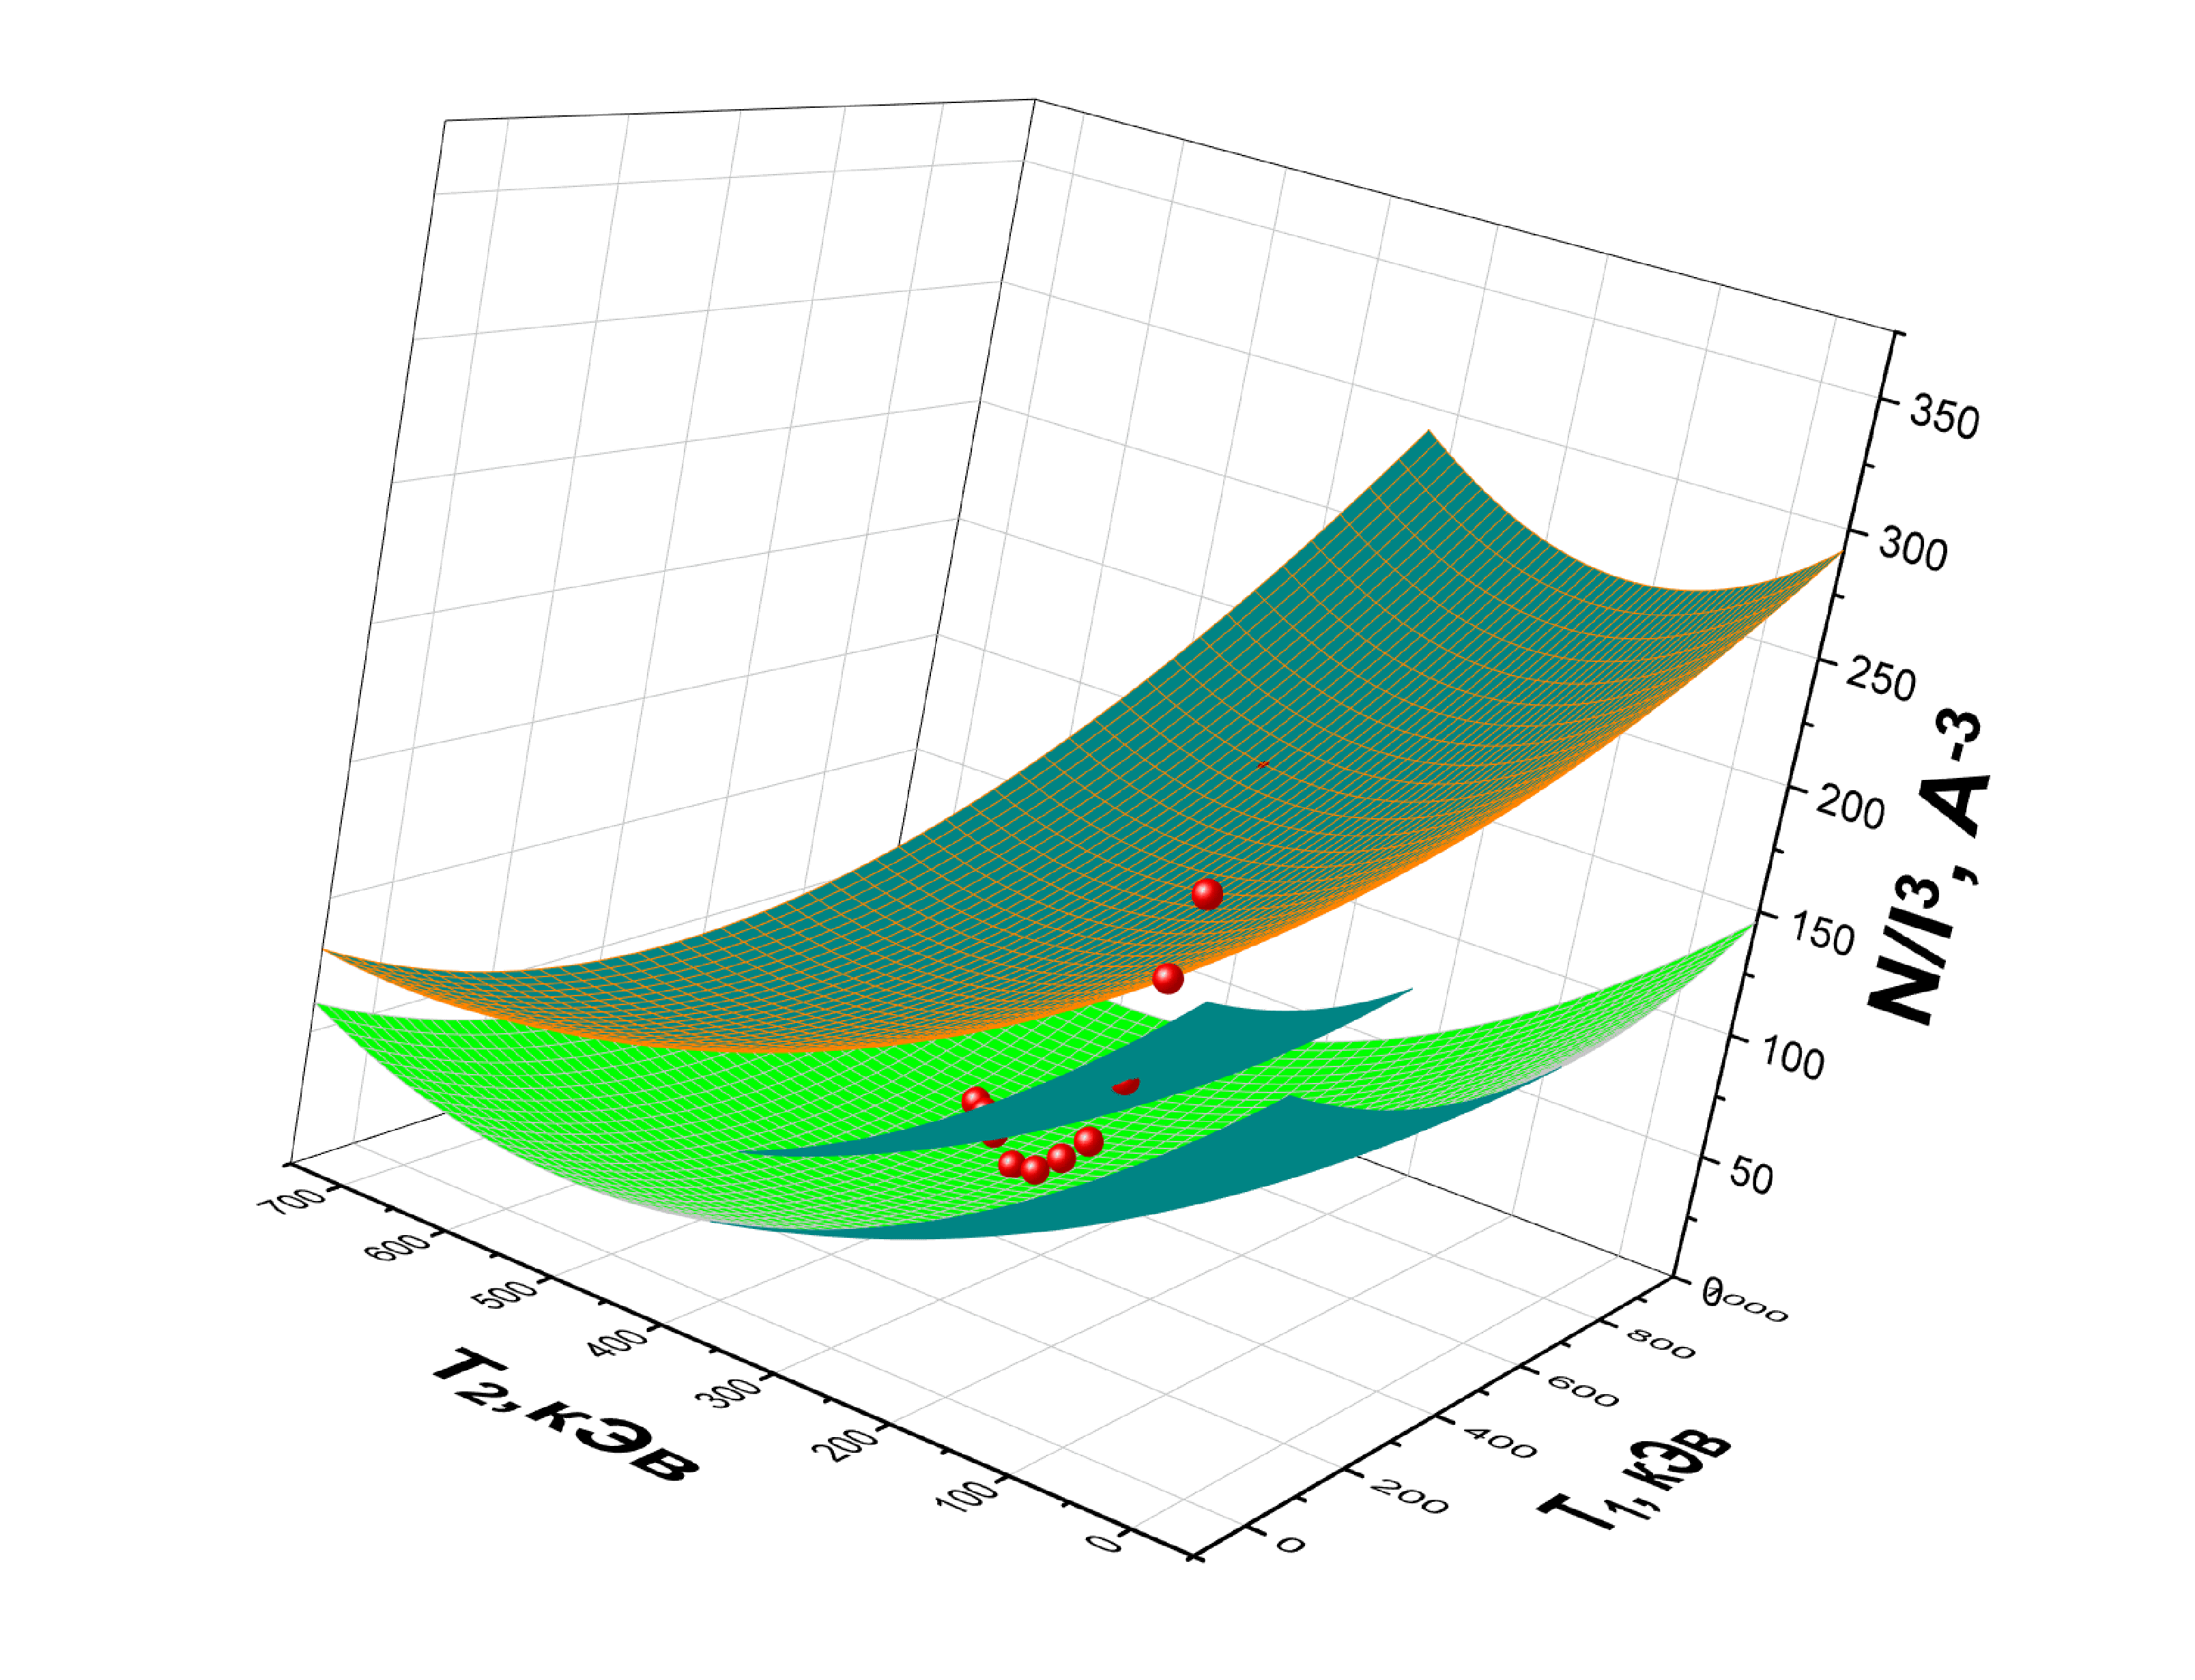
\includegraphics[width=0.8\linewidth]{graph7}
	\caption{Графики, для оценки погрешности $T_{max}$. Верхняя кривая -- $T_{max} = 800 \ кЭв$, нижняя -- $T_{max} = 500 \ кЭв$. Другой ракурс.}
\end{figure}

\pagebreak

Следовательно:

$$
	T_{max} = (698 \pm 100) кЭв
$$

\section*{Определение массы нейтрино}

Сравним максимальную энергию электрона с разностью масс покоя родительского и дочернего ядра.Из закона сохранения энергии:

\begin{align*}
	m_{^{137}Cs}c^2 = m_{^{137}Ba}c^2 + T_{max} +  m_e c^2 + m_{\nu} c^2 \Rightarrow m_{\nu}c^2 \approx (751 \pm 107) кЭв
\end{align*}

\section*{Выводы}

В ходе лабораторной работы мы проанализировали полученный $\beta$-спектр $^{137}Cs$ и двумя разными способами получили максимальную энергию электронов:

\begin{align*}
	T_{max1} = (535 \pm 40) \ кЭв \\
	T_{max2} = (698 \pm 100) \ кЭв
\end{align*}


\end{document}